\section{Abstract}

\begin{figure}
\centering
\includegraphics[width=\textwidth]{images/graphicalabstract.pdf}
\caption{This is a graphical representation of the work completed here, which found a novel role for NFAT activation downstream of macrophage-mycobacterial surface interactions that facilitated the production and secretion of VEGFA to drive angiogenesis.}
% Provide a label so we can cross-reference it from the tex
\label{figure:graphicalabstract}
\end{figure}

As introduced in the previous chapters, pathogenic mycobacteria manipulate the host immune response to generate a productive infection that enables them to transmit to new hosts. To do so, they must both subvert protective immune responses and agonize the pathways that provide them benefit in the way of nutrients, susceptible host cells, or routes of transmission. This necessitates the engagement of both the immune cells themselves and the surrounding stromal cells, all of which much be subverted to generate the optimal pro-bacterial response. One of the mechanisms by which this can occur is through a specific modification of the specialized cell wall lipid, trehalose 6-6'-dimycolate (TDM). This mycobacterial glycolipid has been found to direct angiogenesis toward nascent granulomas to enhance overall bacterial burden. The present study utilizes the zebrafish-\textit{Mycobacterium marinum} infection model to define the signaling basis of the host angiogenic response. Through intravital imaging and targeted, cell-specific peptide-based inhibition, we identify macrophage-specific activation of NFAT signaling as essential to TDM-mediated angiogenesis in vivo.  Exposure of human cells to \textit{Mycobacterium tuberculosis} results in robust induction of VEGFA that is dependent on a signaling pathway downstream of host TDM detection and culminates in NFATC2 activation. As granuloma-associated angiogenesis is known to serve bacterial-beneficial roles, these findings identify potential host targets to improve tuberculosis disease outcomes.

\section{Introduction}

The host rejoinder to infection is driven by an intricately regulated, but occasionally discordant or maladaptive, immune response to pathogenic stimuli at the cell-intrinsic, innate, and adaptive levels \citep{Iwasaki2010, Finlay2006, Haldar2015, MacMicking2004, MacMicking2012, Kim2012}. Although an inflammatory immune response is essential to host survival and pathogen killing, an overly robust response is clearly deleterious to the host, as seen in sepsis \citep{Finethy2020}. However, as we have been in previous chapters, the inflammatory response can also serve pro-bacterial purposes, rendering the immune response impotent. The contributions of immune cells to host defense have been widely studied, but there is growing appreciation for the contributions made my non-immune populations, including stromal cells and the endothelium \citep{Honan2021, Worrell2021, Amersfoort2022, Honan2021} make in shaping the host response to both acute and chronic infections \citep{Mueller2009, Randow2013, Krishnamurty2020}. Pathogens have long been known to possess sophisticated mechanisms to undermine signaling pathways in immune cells and, more recently, have been shown to manipulate development and homeostatic tissue processes to force them toward pathogen-beneficial states \citep{Menzies1998, Guichard2013}.

\textit{Mycobacterium tuberculosis} is among history's most widespread and successful pathogens. It has evolved an array of sophisticated mechanisms that manipulate its human host to enable bacterial survival, replication, and transmission. Upon infection, \textit{M. tuberculosis} sets in motion an intricate immune response wherein innate immune cells, consisting initially of macrophages, congregate at the bacterial focus and then undergo an epithelioid transformation and interdigitate to form an encased granuloma, the hallmark feature of tuberculosis, which provides both the replicative niche and the major host-pathogen interface of tuberculosis disease \citep{Cronan2016, Pagan2018, Cronan2021}. Granuloma-associated vasculature has long been noted in human and animal models of TB \citep{Cudkowicz1952, Russell2010} but the mechanisms of induction and precise contributions to infection are not yet fully understood.

Many of the major pathological features of mycobacterial granulomas, including associated vascularization, are conserved from zebrafish to humans \citep{Swaim2006, Bohrer2021}. Zebrafish can be infected with a natural pathogen, \textit{Mycobacterium marinum}, which induces a robust angiogenic response during granuloma formation in both the larva and adult. This process, much like that in humans, non-human primates, and rabbits, is associated with production of a pro-angiogenic chemokine, Vegfaa, at the site of infection \citep{Oehlers2015}. This chemokine has long been known to be a critical regulator of angiogenesis in both developmental and pathological contexts \citep{Chung2011, Leung1989, Adams2007}. Similarly, human granulomas have been shown to express VEGFA and are physically associated with blood vessels that penetrate the outer granulomatous layers \citep{Datta2015}. Subsequent work has demonstrated a role for these vessels in supporting bacterial growth and in dissemination of the bacilli from their primary site of infection \citep{Polena2016}. Additional roles for VEGFA in non-angiogenic processes have also been noted, suggesting that angiogenic signaling cascades can also alter the biology of granuloma macrophages to improve disease outcomes \citep{Harding2019}. Additional roles have been proposed for the related lymphangiogenesis \citep{Alitalo2005, Duong2012, Lerner2020}, where pharmacological blockade of these vessels of the lymphatic system also offer host-protective benefits \citep{Harding2015}. Recent profiling of human and non-human primate granulomas have confirmed the presence of aberrant vasculature associated with \textit{M. tuberculosis} granulomas \citep{Gideon2022, McCaffrey2022, Cronan2021}.

Pathogenic mycobacteria have evolved specialized mechanisms to promote and accelerate angiogenesis. Notably, the extensively modified and essential outer cell envelope component trehalose 6-6'-dimycolate (TDM) is cis-cyclopropanated by the enzyme PcaA \citep{Glickman2000, Rao2005}. Mutation of pcaA results in a reduction in granuloma angiogenesis and concomitant reduction in bacterial burden; correspondingly, cyclopropanated TDM alone is sufficient to induce host angiogenesis \citep{Saita2000, Sakaguchi2000, Walton2018}. As \textit{pcaA}-dependent vascularization supports bacterial growth, factors driving angiogenesis represent potential sites of therapeutic intervention yet the signals that mediate this host process remain unclear.

TDM is an extraordinarily long-chain, hydrophobic (C\textsubscript{60}-C\textsubscript{100}) glycolipid \citep{Noll1956a, Noll1956b, Hunter2006a, Behling1993} that has been shown to be detected in cell culture and murine models by host C-type lectin receptors, most notably MCL (CLEC4D) and MINCLE (CLEC4E), as well as by Toll-like receptor 2 (TLR2), CD14, and MARCO \citep{Bowdish2009, Matsunaga2009, Miyake2013, Ishikawa2009}. Canonically, C-type lectin signaling is transmitted through a CARD9-NF-$\upkappa$B signaling pathway that results in the transcription and production of TNF-$\upalpha$, IL-1$\upbeta$, IL-6 and other cytokines \citep{Yamasaki2008, Goodridge2009, LobatoPascual2013, Zhao2014, Deerhake2021}. However, beyond CARD9, a number of other downstream signaling pathways are engaged by C-type lectin activation and likely control discrete aspects of signaling \citep{Goodridge2007, Deerhake2021}.

Here, we synthesize findings from zebrafish and cell culture models to define the \textit{in vivo} angiogenic response induced by pathogenic mycobacteria. Contrary to classical models of C-type lectin signaling, we find that cis-cyclopropanated TDM exerts its pro-angiogenic effects through an alternative NFAT-driven pathway rather than canonical CARD9-NF-$\upkappa$B signaling. We use peptide-mediated, cell-specific inhibition of NFAT to demonstrate that both early and mature granuloma angiogenesis are dependent upon macrophage-NFAT signaling. We identify \textit{NFATC2} as the predominant isoform mediating \textit{VEGFA} induction and angiogenesis \textit{in vitro} and \textit{in vivo}. These findings define the basis of granuloma-associated angiogenesis during pathogenic mycobacterial infections and suggest new targets for host-directed therapeutic interventions during tuberculosis.

\section{Results}

\subsection{Macrophage Induction of \textit{vegfaa} and Angiogenesis during Mycobacterial Infection}

\begin{figure}
\centering
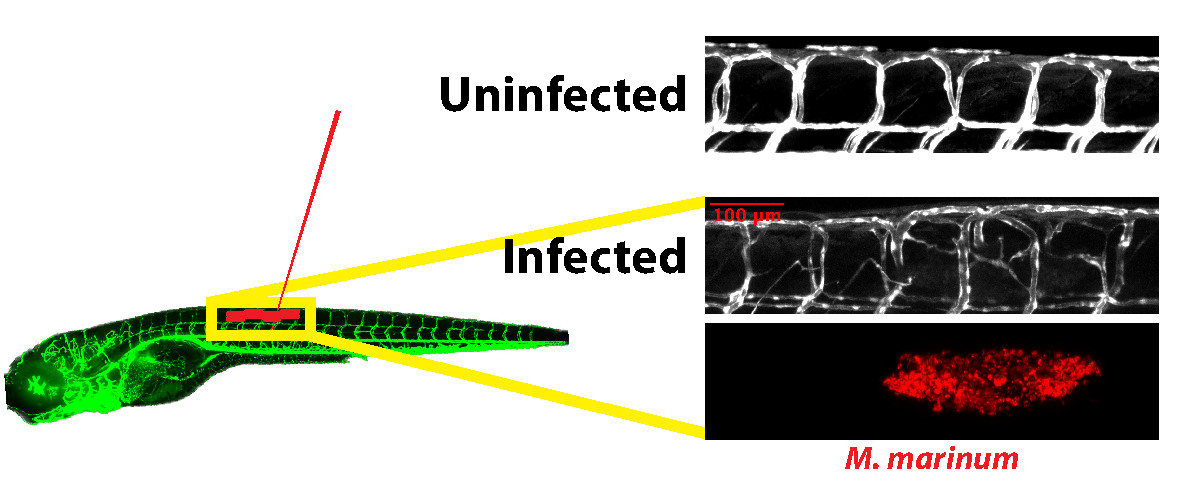
\includegraphics[width=\textwidth]{images/angexample.pdf}
\caption{Pictorial representation of the site of infection and angiogenic outcomes from infection. After injection into a peri-notochordal space along the trunk of the fish, the bacteria replicate and blood vessels grow toward the site of infection, as compared to the uninfected reference.}
% Provide a label so we can cross-reference it from the tex
\label{figure:angexample}

\end{figure}

Injection of live \textit{Mycobacterium marinum} into the dorsal trunk of the zebrafish larva is sufficient to induce a robust angiogenic response adjacent to nascent granulomas in a macrophage-dependent manner \citep{Oehlers2015} (\autoref{figure:angexample}). The stereotyped vasculature along this region of the larva allows facile quantitation of neovascularization during and after granuloma formation or other insult \citep{Lawson2002, Jin2005, Gore2012, Matsuoka2018}. We demonstrated previously that cis-cyclopropanated trehalose 6-6'-dimycolate (TDM) is required for the induction of \textit{vegfaa} and angiogenesis at the site of infection. Furthermore, we found that genetic blockade of Vegfaa signaling was sufficient to abolish angiogenesis during infection with wild-type mycobacteria \citep{Walton2018}. Taken together, these findings suggest that the failure to induce \textit{vegfaa} is a primary contributor to the loss of angiogenesis in \textit{pcaA}-deficient granulomas.

\begin{figure}
\centering
\includegraphics[width=\textwidth]{images/extracellularvegfa.pdf}
\caption{Around 60 hours post infection, macrophages interacting with the extracellular bacteria at the site of infection begin to express \textit{vegfaa}, as reported by the \textit{vegfaa}:\textit{eGFP\textsuperscript{pd260}} transgene. In (A), a time series can be seen showing \textit{vegfaa}-expressing macrophages and in (B), macrophages can be seen engaging with what appears to be extracellular bacteria that has accumulated over the course of the infection.}
% Provide a label so we can cross-reference it from the tex
\label{figure:ecvegfa}

\end{figure}

To study this phenomenon further, we began by examining the kinetics of \textit{vegfaa} induction to identify the cellular source of Vegfaa during granuloma formation. To test whether macrophages were playing this role, we developed a macrophage-specific reporter using the previously described \textit{acod1} promoter (also known as \textit{irg1}), Tg(\textit{irg1}:\textit{tdTomato\textsuperscript{xt40}}) (from here, \textit{irg1}:\textit{tdTomato}). \textit{irg1} has been found to be expressed specifically in zebrafish macrophages and is upregulated during infection \citep{Sanderson2015, Kwon2022}. We then crossed this line with the \textit{vegfaa} reporter line TgBAC(\textit{vegfaa}:\textit{eGFP\textsuperscript{pd260}}) (\textit{vegfaa}:\textit{eGFP} throughout) \citep{Karra2018} and infected double transgenic \textit{irg1}:\textit{tdTomato}; \textit{vegfaa}:\textit{eGFP} progeny with \textit{M. marinum} expressing eBFP2 (\textit{Mm}-eBFP2) to simultaneously visualize bacteria, macrophage localization, and \textit{vegfaa} production \textit{in vivo} \citep{Takaki2013}.

\begin{figure}
\centering
\includegraphics[width=\textwidth]{images/extracellularflk1.pdf}
\caption{At later time points, after \textit{vegfaa} induction, blood vessels proliferate and begin to grow toward the site of infection in association with nearby macrophages. (A) shows this process occurring over the time period studied and culminating in a new vessel nearly spanning the intersomitic vasculature. (B) displays the accumulation of extracellular bacteria and macrophage killing over this time period.}
% Provide a label so we can cross-reference it from the tex
\label{figure:ecflk1}

\end{figure}

We began imaging at a time point that preceded robust induction of \textit{vegfaa}:\textit{eGFP} but would allow us to capture the maximum time span of these events. We observed an increase in \textit{vegfaa} reporter signal over time that appeared largely localized to macrophages (\autoref{figure:ecvegfa}A). We observed that bacteria initially grew primarily intracellularly within individual macrophages at 36 hours post infection but began to grow in characteristic extracellular cords by approximately 84 hours post infection with little to no intracellular containment at this site by 96 hours post infection (\autoref{figure:ecvegfa}B). The increase in extracellular growth coincided with the induction of eGFP signal in macrophages at ~64 hours (\autoref{figure:ecvegfa}A), suggesting that, at low overall burden, intracellular detection is unable to induce \textit{vegfaa} expression while extracellular engagement correlates with \textit{vegfaa} expression during early stages of granuloma formation (\autoref{figure:ecvegfa}). 

We next visualized the production of angiogenic vessels throughout infection in parallel to our characterization of \textit{vegfaa} induction. Due to an inability to separate discrete emission wavelengths using two GFP reporter lines, we were unable to examine all four components (bacteria, \textit{vegfaa} induction, macrophages, and vasculature) simultaneously. To relate this process directly to the angiogenesis observed in mycobacterial granulomas, we crossed the \textit{irg1}:\textit{tdTomato} macrophage reporter to the Tg(\textit{kdrl}:\textit{eGFP\textsuperscript{s843}}) (from here, \textit{kdrl}:\textit{eGFP}) line, which labels vascular endothelium (\textit{irg1}:\textit{tdTomato}; \textit{kdrl}:\textit{eGFP}) \citep{Jin2005}. Under the same conditions and burden at which we infected the \textit{vegfaa} and macrophage dual reporter line, we observed robust vascularization at approximately 96 hours post-infection, subsequent to initial granuloma formation and \textit{vegfaa} induction (\autoref{figure:ecflk1}A, B). 

\subsection{Genetic \textit{card9} Deficiency Does Not Compromise Angiogenesis During Mycobacterial Infection}

\begin{figure}
\centering
\includegraphics[height=2in]{images/JB96_myd88_TDM_103022.png}
\caption{\textit{myd88} is dispensable for angiogenesis during infection, suggesting a TLR- and IL-1R-independent signaling pathway is necessary for inducing angiogenesis downstream of TDM detection. Larval zebrafish were injected with IFA or TDM, imaged and quantitated, and then matched to genotype. Adapted from personal contributions to \citet{Walton2018}.}
% Provide a label so we can cross-reference it from the tex
\label{figure:myd88}

\end{figure}

Given these observations suggesting that macrophages engaging extracellular bacteria are an important source of \textit{vegfaa} expression, we interrogated pattern recognition receptor (PRR) signaling pathways that had been implicated in host responses to TDM, a major external component of the mycobacterial cell envelope. We had previously found that \textit{myd88} was dispensable for the induction of angiogenesis in response to TDM \textit{in vivo }\autoref{figure:myd88} \citep{Bowdish2009, Walton2018}. This suggested that the described TLR2-mediated responses that function downstream of TDM detection in some contexts were unlikely to be required for this process \footnote{This could not, however, rule out any potential role for CD14-mediated signaling independent of TLR2. One issue is that the zebrafish do not have an identified CD14 homolog, but additional data clarifies things somewhat.}. Rather, we found that the Fc$\upgamma$R homologs in zebrafish, \textit{fcer1g} and \textit{fcer1gl}, are required for the full angiogenic response to TDM \citep{Walton2018}, implicating C-type lectin receptors signaling in mediating this response \citep{Richardson2014, Zhao2014}.

\begin{figure}
\centering
\includegraphics[width=\textwidth]{images/card9.pdf}
\caption{\textit{card9}, the canonical downstream adaptor from C-type lectin signaling, is not required for angiogenesis during mycobacterial infection. (A), (C), and (D) show three replicates of this experiment from genotype-blind experiments. (B) shows a representative example of the effect seen, where no differences can be ascertained between genotypes. (E) displays the 28 base pair insertion generated, with the new early stop codon highlighted in red.}
% Provide a label so we can cross-reference it from the tex
\label{figure:card9}
\end{figure}

As many of the downstream activities of C-type lectin receptors have been ascribed to the activation of CARD9-NF-$\upkappa$B signaling \citep{Goodridge2009, LobatoPascual2013, Zhao2014, Williams2017, Deerhake2021}, we assessed what role this pathway might play in angiogenesis during mycobacterial infection. We developed a \textit{card9} knockout zebrafish line using CRISPR/Cas9 that carries a 28 bp insertion, resulting in an early stop after 59 amino acids (\textit{card9\textsuperscript{xt31}}) (\autoref{figure:card9}E). We then assayed these animals in the \textit{kdrl}:\textit{eGFP} transgenic background by incrossing \textit{kdrl}:\textit{eGFP}; \textit{card9\textsuperscript{xt31/+}} animals and infecting the resulting offspring with tdTomato-fluorescent \textit{M. marinum} (\textit{Mm}-tdTomato) at 2 days post fertilization (dpf) \citep{Jin2005, Oehlers2015}(\autoref{figure:card9}A, B). We quantitated the resulting aberrant vasculature at 4 days post-infection (dpi) under genotypic blinding and post hoc matched these measurements to genotype. To our surprise, there were no significant differences between the three genotypes across three independent replicates (\autoref{figure:card9}A, C, D), suggesting either redundancy between multiple established pathways or the existence of an alternative pathway downstream of TDM detection that was \textit{fcer1g}/\textit{fcer1gl}-dependent, but independent of both \textit{myd88} and \textit{card9}. 

\subsection{Pharmacological Inhibition of NFAT Activation Limits Angiogenesis in Response to Mycobacteria and TDM}

\begin{figure}
\centering
\includegraphics[width=\textwidth]{images/fk506inf.pdf}
\caption{Treatment of infected larval zebrafish with the calcineurin-NFAT inhibitor FK506 at 125nM results in a reduction in infection-induced angiogenesis, suggesting a role for this pathway in inducing angiogenesis during infection.}
% Provide a label so we can cross-reference it from the tex
\label{figure:fk506inf}
\end{figure}

Although many of the physiological consequences of C-type lectin receptor induction are often ascribed to CARD9-NF-$\upkappa$B signaling, this PRR class is also known to activate a distinct transcription factor family with known roles in immunity --€“ the nuclear factor of activated T cells, or NFAT \citep{Goodridge2007, Deerhake2021}. This calcium-responsive transcription factor pathway is best described in its role regulating T cell biology, but there are numerous reports describing various roles for the members of this pathway in other cell types, including macrophages (see \autoref{NFAT}) \citep{Symes1998, Jones2000, Crabtree2002, Horsley2002, Elloumi2012}. Given that there are four mammalian members of this pathway and six zebrafish homologs with potentially overlapping functions, we began with a pharmacological approach to globally inhibit NFAT signaling through all six zebrafish isoforms. Although this comes with caveats with specificity -- as described in \autoref{nfatc1}, NFATC1 has important roles in angiogenesis within the endothelium -- it offers an opportunity to assess the general roles of this pathway as a first-pass approach. 

\begin{figure}
\centering
\includegraphics[width=\textwidth]{images/fk506tdm.pdf}
\caption{Treatment of infected larval zebrafish with the calcineurin-NFAT inhibitor FK506 at 125nM results in a reduction in TDM-induced angiogenesis, suggesting a role for NFAT signaling in inducing TDM-dependent pro-angiogenic signaling.}
% Provide a label so we can cross-reference it from the tex
\label{figure:fk506tdm}
\end{figure}

We first infected 2 days post fertilization \textit{kdrl}:\textit{eGFP} larval zebrafish with \textit{Mm}-tdTomato in the trunk and treated them with 125 nM FK506, a clinically utilized calcineurin inhibitor that blocks NFAT activation, for the duration of the experiment \citep{Ellis1995}. This modest dose of FK506 was chosen due to developmental toxicities observed at higher doses in my hands and is in line with the dosage used by others \citep{Kujawski2014}. We imaged the fish at 4 days post infection and quantitated the degree of vasculature induced in the presence and absence of inhibitor under computational blinding. Even with at this low dose of FK506, we noted a small, but statistically significant reduction in the mean degree of neovascularization at this time point, consistent with a role for NFAT in controlling angiogenesis in response to \textit{M. marinum} infection (\autoref{figure:fk506inf}A, B) \citep{Kujawski2014}. To ask whether this effect was specific to recognition of TDM, we injected purified TDM or vehicle (incomplete Freund's adjuvant; IFA) alone into the trunks of 2 days post fertilization larvae. Treatment with FK506 resulted in a statistically significant reduction in the degree of angiogenesis induced at 2 days post injection (\autoref{figure:fk506tdm}A, B), suggesting that this pathway was specifically relevant to TDM-dependent angiogenesis.

\subsection{The Isoform \textit{nfatc2a} is Specifically Required for Angiogenesis During Infection}

\begin{figure}
\centering
\includegraphics[width=\textwidth]{images/mosaicnfatc3a.pdf}
\caption{Assays in mosaic, CRISPR/Cas9 RNP-injected larval zebrafish suggested that \textit{nfatc3a} was dispensable for the induction of angiogenesis during infection. Panels (A), (B), (C) show the results of three replicates of these mosaic injections. (D) shows the results of the same assay in a stable knockout background of \textit{nfatc3a}, confirming the preliminary results from the mosaic assay. (E) shows the nature of the mutation in \textit{nfatc3a\textsuperscript{xt59}}.}
% Provide a label so we can cross-reference it from the tex
\label{figure:mosaic}
\end{figure}

Combining our observations on the correspondence of granuloma formation and the induction of \textit{vegfaa} with our data implicating the NFAT pathway, we sought to identify NFAT isoforms that were enriched in granuloma macrophage populations. Aside from investigations made into \textit{nfatc1}, which is restricted to the endocardium, lymphatic vessels, and the notochord during much of zebrafish development (see \autoref{nfatc1}) \citep{Pestel2016, Shin2019, Bagwell2020}, little is known of the expression patterns of these genes in zebrafish\footnote{As mentioned previously in \autoref{nfatc4}, the NFATC4 isoform is thought to not be expressed in the hematopoietic compartment, an observation backed up by some more recent data as well \citep{Peuker2022}.}, especially in the context of infection. We first made use of published scRNA-seq datasets from mycobacterial granulomas in zebrafish and non-human primates for \textit{nfat} transcripts that were robustly expressed in granuloma macrophages at the population level and identified both zebrafish \textit{nfatc2a} and \textit{nfatc3a} as plausible candidates \citep{Cronan2021, Gideon2022}.

To examine potential roles for \textit{nfatc2a} and \textit{nfatc3a} in granuloma-associated angiogenesis in vivo, we first screened F\textsubscript{0} CRISPR-injected mosaic knockouts (``crispants'') to rapidly evaluate these candidate genes. Using this approach, similar to that used previously by other groups, we assessed the relative roles of these two isoforms individually and in tandem, measuring the angiogenic response to mycobacterial infection in the \textit{kdrl}:\textit{eGFP} background \citep{Jao2013, Hoshijima2016, Wu2018, Hoshijima2019, Kroll2021}. We found that \textit{nfatc2a} inhibition resulted in a $\sim$50-80\% reduction in angiogenesis (\autoref{figure:mosaic}A-C). In contrast, \textit{nfatc3a} had no effect on the length of ectopic blood vessels present (\autoref{figure:mosaic}A-C). The dual targeted double mosaics were statistically indistinguishable from the \textit{nfatc2a} injected fish alone (\autoref{figure:mosaic}A-C). This allowed us to prospectively identify \textit{nfatc2a} as an NFAT isoform required for full angiogenic response to mycobacteria while \textit{nfatc3a}, despite expression in overlapping cell populations, appeared to be entirely dispensable for this process at this point in time (\autoref{figure:mosaic}A-C). 

\begin{figure}
\centering
\includegraphics[width=\textwidth]{images/nfatc2alarvae.pdf}
\caption{\textit{nfatc2a} is required for the angiogenic response to infection. Use of the stable mutant line \textit{nfatc2a\textsuperscript{xt69}} demonstrated an important role for this pathway in inducing angiogenesis. (A) diagrams the mutation I established. (B), (C) and (D) show three replicates of the infection experiment, demonstrating robust and reproducible reduction in angiogenesis in both the heterozygous and mutant conditions relative to wild-type. (E) shows a representative example of the effect seen, with robust angiogenesis under wild-type conditions and a significant reduction with \textit{nfatc2a\textsuperscript{xt69/xt69}}.}
% Provide a label so we can cross-reference it from the tex
\label{figure:c2larvae}
\end{figure}

We then established stable, germline transmitting indel mutant alleles for both genes to validate our results from mosaic animals. Recapitulating our results in the F0 generation, the \textit{nfatc3a\textsuperscript{xt59}} mutation carrying a 22 bp deletion (leading to an early stop codon at amino acid 9 in exon 1) had no effect on angiogenesis at 4 days post infection (\autoref{figure:mosaic}D, E). We then developed a knockout line of \textit{nfatc2a} bearing a net 4 bp insertion leading to an early stop codon in the second exon (at amino acid 273, frameshifted after amino acid 247), prior to the DNA-binding domain (\textit{nfatc2a\textsuperscript{xt69}}) (\autoref{figure:c2larvae}A). We repeated our angiogenesis assay using larvae from in-crosses of \textit{kdrl}:\textit{eGFP}; \textit{nfatc2a\textsuperscript{xt69/+}} animals that produced expected Mendelian ratios of wild-type, heterozygous, and homozygous mutant offspring. Consistent with the results from mosaic animals, homozygous knockout of \textit{nfatc2a} was sufficient to reduce the degree of angiogenesis present in larval zebrafish at 4 days post infection (\autoref{figure:c2larvae}B-E). Importantly, given the known role of NFAT isoforms in T cell function, these defects emerged prior to the developmental emergence of functional T cells, which does not occur until approximately 6 days post fertilization as the thymus develops \citep{Trede2004}. However, whole animal knockouts could not address potential roles for cell types other than macrophages in mediating this process. 

\subsection{Macrophage-NFAT is Essential for Angiogenesis Induction \textit{in vivo}}

\begin{figure}
\centering
\includegraphics[width=\textwidth]{images/vivitconstruct.pdf}
\caption{Design of the \textit{irg1}:\textit{VIVIT-tdTomato} construct. (A) shows the overall layout of the construct, with \textit{irg1} driving the expression of the VIVIT peptide conjugated to tdTomato. (B) shows a representative \textit{irg1}:\textit{VIVIT-tdTomato\textsuperscript{xt38}} larva.}
% Provide a label so we can cross-reference it from the tex
\label{figure:vivitdiagram}
\end{figure}

Given our observations on \textit{vegfaa} induction in macrophages at the granuloma, we tested whether NFAT signaling was required specifically in macrophages for granuloma-associated angiogenesis. For \textit{in vivo} inhibition of macrophage NFAT signaling during infection, we applied an approach that takes advantage of the NFAT-inhibitory peptide VIVIT which competitively inhibits calcineurin-dependent activation of all the NFATc isoforms \citep{Aramburu1999}. This approach has been successfully used as an exogenous treatment in cell culture \citep{Deerhake2021} and mice \citep{Noguchi2004, Elloumi2012, Rojanathammanee2015}, through ectopic overexpression in cell culture \citep{McCullagh2004},  and, more recently, in mice \citep{Poli2022, Peuker2022}. We developed a transgenic zebrafish line in which VIVIT is expressed specifically in macrophages, Tg(\textit{irg1}:\textit{VIVIT-tdTomato\textsuperscript{xt38}}) (from here, simply \textit{irg1}:\textit{VIVIT}) (\autoref{figure:vivitdiagram}A, B) \citep{Sanderson2015}. We assessed whether the macrophage-specific expression of VIVIT would be sufficient to reduce the degree of angiogenesis during infection in the trunk with wild-type \textit{M. marinum} expressing mCerulean (\textit{Mm}-mCerulean). We found that macrophage-specific VIVIT expression significantly reduced angiogenesis in response to infection (\autoref{figure:vivitinf}A-D). This suggested a macrophage-specific role for NFAT signaling downstream of mycobacterial detection that was necessary to induce angiogenesis, presumably through the \textit{nfatc2a} isoform.

\begin{figure}
\centering
\includegraphics[width=\textwidth]{images/vivitlinf.pdf}
\caption{Macrophage-specific VIVIT expression in larval zebrafish inhibits infection-induced angiogenesis. (A), (B), and (C) show three replicates of this infection experiment and a robust reduction in the amount of angiogenesis with expression of the VIVIT peptide compared to \textit{irg1}:\textit{tdTomato}-only controls. (D) shows representative images o the effect observed, with reduced angiogenesis seen in the VIVIT condition.}
% Provide a label so we can cross-reference it from the tex
\label{figure:vivitinf}
\end{figure}

To ask more directly whether the decreased angiogenesis observed in the NFAT-deficient macrophages was via the TDM-mediated pathway, we used the TDM injection assay we had developed previously. We injected TDM or the IFA vehicle into the trunk of 2 days post fertilization larval zebrafishand measured the resulting angiogenesis at 2 days post injection \citep{Walton2018}. TDM was sufficient to induce angiogenesis \textit{in vivo} and this effect was dependent upon functional NFAT signaling, with the degree of TDM-induced angiogenesis reduced to the level of the vehicle alone in \textit{irg1}:\textit{tdTomato} animals compared to \textit{irg1}:\textit{tdTomato} controls (\autoref{figure:vivittdm}A-D).

\begin{figure}
\centering
\includegraphics[width=\textwidth]{images/vivittdm.pdf}
\caption{Macrophage-specific VIVIT expression reduces TDM-induced angiogenesis in the larval zebrafish. (A), (B), and (C) display three independent replicates of this experiment; (D) demonstrates the effect by representative images showing the reduction seen in the VIVIT-expressing condition.}
% Provide a label so we can cross-reference it from the tex
\label{figure:vivittdm}
\end{figure}

\subsection{NFAT Activation is Essential for Angiogenesis in Adult Granulomas}\label{nfatc2aAdult}

\begin{figure}
\centering
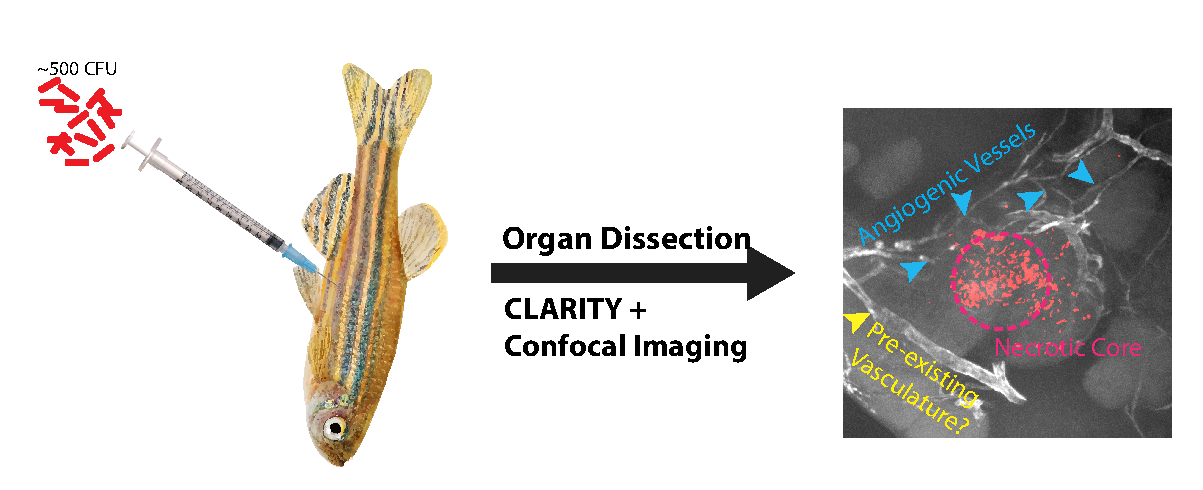
\includegraphics[width=\textwidth]{images/adultinf.pdf}
\caption{Schematic of the infection and CLARITY-clearing approach used for adult infection experiments. Adult zebrafish (>12 weeks post fertilization) are infected interperitoneally with ~500 CFU of fluorescent \textit{M. marinum} and then organs are harvested and fixed approximately 14 days later, cleared with detergent, and then imaged.}
% Provide a label so we can cross-reference it from the tex
\label{figure:adult}
\end{figure}

Adult zebrafish are equipped with both innate and adaptive immunity and form mycobacterial granulomas that histologically mirror epithelioid human tuberculosis granulomas \citep{Swaim2006}, including induction of a surrounding vascular network. To assess whether our findings in the larvae translated to a longer-term context in the presence of adaptive immunity, we infected adult \textit{kdrl}:\textit{eGFP}; \textit{nfatc2a\textsuperscript{xt69/xt69}} zebrafish and \textit{kdrl}:\textit{eGFP}; \textit{nfatc2a\textsuperscript{+/+}} siblings with \textit{Mm}-tdTomato and examined their peritoneal organs at 18 days post infection after CLARITY-based clearing \citep{Chung2013, Cronan2015}. Cleared organs were then imaged by spinning disk confocal microscopy (\autoref{figure:adult}). We measured the total vascular network surrounding the granulomas in a programmatically blinded fashion \citep{Salter2016} and \autoref{blinders} and found that \textit{nfatc2a\textsuperscript{xt69/xt69}} fish had a significant reduction (${\sim}$50\%) in the length of the vascular network compared to wild-type siblings, further validating this gene as important for the angiogenic response \textit{in vivo} (\autoref{figure:c2adult}A-D). These putatively neovascular vessels tend to be highly branched and to be comprised of a limited number of cells with small or non-existent luminal volume, indicating that they are still in the sprouting stage of angiogenesis and suggesting a potential failure to mature over time. We observed robust effects that are likely understated in our quantitation, as we could not formally make any distinction between thicker, existing vasculature present at baseline that happens to fall nearby the granuloma and the characteristic neovascularization more intimately associated with the granuloma and present in wild-type but reduced in \textit{nfatc2a} mutants (\autoref{figure:grandiv}).

\begin{figure}
\centering
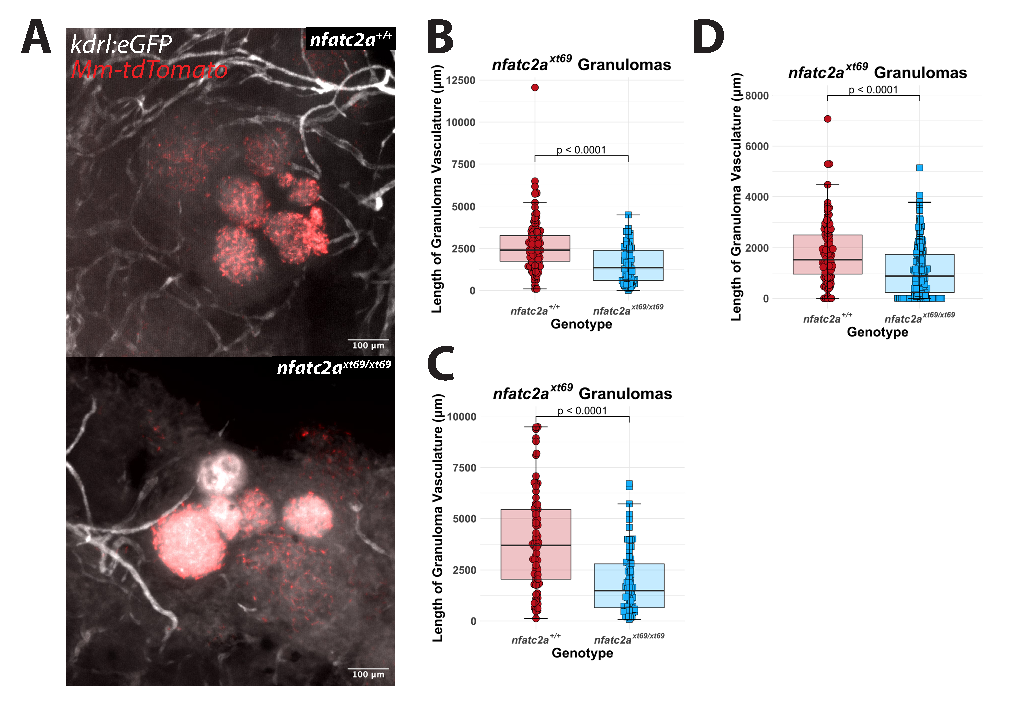
\includegraphics[width=\textwidth]{images/nfatc2aadult.pdf}
\caption{\textit{nfatc2a} is required for robust angiogenesis in established granulomas. (A) shows images comparing wild-type and \textit{nfatc2a\textsuperscript{xt69/xt69}} granulomas and a substantial reduction in the overall angiogenic effect can be seen. This is quantitated in (B), (C), and (D), with an ~50\% reduction in the total vasculature visible in the proximity of each granuloma.}
% Provide a label so we can cross-reference it from the tex
\label{figure:c2adult}
\end{figure}

\begin{figure}
\centering
\includegraphics[width=\textwidth]{images/grandiv.pdf}
\caption{Mycobacterial granulomas display significant heterogeneity in vascularization and many are in physical proximity to mature, likely pre-existing vessels. One of the drawbacks of the adult angiogenesis measurements is significant background seen in the proximity of these granulomas, as seen in this figure.}
% Provide a label so we can cross-reference it from the tex
\label{figure:grandiv}
\end{figure}

\subsection{\mbox{Macrophage-specific} NFAT Inhibition in Mature Granulomas Reduces Angiogenesis}

We next evaluated whether macrophage-specific NFAT inhibition had similar effects on vascularization in adult zebrafish. We infected adult \textit{irg1}:\textit{tdTomato}; \textit{kdrl}:\textit{eGFP} and \textit{irg1}:\textit{VIVIT-tdTomato}; \textit{kdrl}:\textit{eGFP} double transgenic zebrafish with \textit{Mm}-mCerulean and examined visceral organs at 14 days post infection. We used confocal imaging to visualize individual CLARITY-cleared organs and measured the total length of granuloma-proximal vasculature under blinding as above (Salter, 2016). We found that the degree of vascularization was significantly reduced around granulomas from \textit{irg1}:\textit{VIVIT-tdTomato} fish as compared to \textit{irg1}:\textit{tdTomato} fish (\autoref{figure:vivitadult}A-D). The extent of the vascular network in the \textit{irg1}:\textit{VIVIT-tdTomato} condition was notably restricted in most cases or solely comprised of more mature, luminal vessels, suggesting a total failure to induce an angiogenic response (\autoref{figure:vivitadult}A). These findings, consistent with our previous data from both larval zebrafish infections in the \textit{irg1}:\textit{VIVIT-tdTomato} background and in the \textit{nfatc2a} mutant adult fish, point to a critical role for macrophage-specific NFAT activation in inducing the angiogenic response at mycobacterial granulomas. Furthermore, this establishes that NFAT function is broadly conserved from early larval infection through to the mature necrotic granulomas that characterize adult infection.

\begin{figure}
\centering
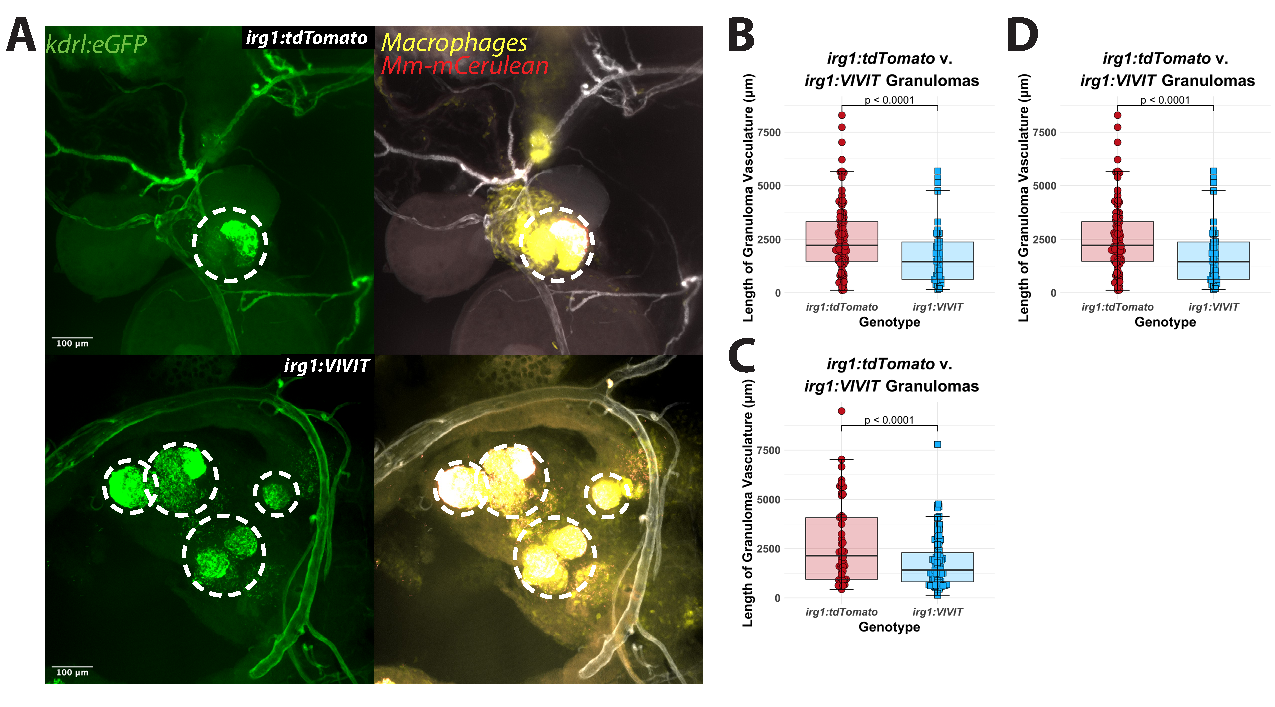
\includegraphics[width=\textwidth]{images/vivitadult.pdf}
\caption{Macrophage-VIVIT expression inhibits granuloma angiogenesis in the adult zebrafish infection model. (A) shows images comparing \textit{irg1}:\textit{tdTomato} and \textit{irg1}:\textit{VIVIT-tdTomato} granulomas and a substantial reduction in the overall angiogenic effect can be seen. This is quantitated in (B), (C), and (D), with an ~50\% reduction in the total vasculature visible in the proximity of each granuloma.}
% Provide a label so we can cross-reference it from the tex
\label{figure:vivitadult}
\end{figure}

\subsection{Inhibition of NFAT Signaling Results in Decreased Bacterial Burden}

We had previously shown that inhibition of granuloma-associated vascularization is associated with decreased bacterial burden. Mycobacterial mutants unable to induce vascularization ($\upDelta$\textit{pcaA}), and either genetic or pharmacological inhibition of VEGF signaling all result in lower bacterial burden, presumably due to functions of the aberrant vasculature promoting bacterial growth and/or inhibiting bacterial killing \citep{Rao2005, Glickman2000, Oehlers2015, Walton2018} or through more direct pro-bacterial activities of VEGFA \citep{Harding2019}. To examine the effect on burden of inhibition of NFAT signaling, we performed colony forming unit (CFU) assays at timepoints after the induction of angiogenesis and granuloma maturation. We infected \textit{nfatc2a\textsuperscript{+/+}} and \textit{nfatc2a\textsuperscript{xt69/xt69}} adult zebrafish with \textit{Mm}-tdTomato and plated them for CFU at 24 days post infection. We found that knockout of \textit{nfatc2a} resulted in a ${\sim}$50\% decrease in median colony number compared to wild-type after extended infection (\autoref{figure:cfu}A). 

\begin{figure}
\centering
\includegraphics[height=3in]{images/cfu.pdf}
\caption{Inhibition of NFAT signaling results in a reduction in mycobacterial CFU at time points after granuloma formation. (A) shows a reduction in bacterial burden in \textit{nfatc2a} mutant fish while (B) shows a similar reduction in burden in VIVIT-expressing fish.}
% Provide a label so we can cross-reference it from the tex
\label{figure:cfu}

\end{figure}

Finally, we evaluated the impact of macrophage-specific NFAT inhibition on whole organism bacterial burden. We infected adult zebrafish possessing either the \textit{irg1}:\textit{tdTomato} or \textit{irg1}:\textit{tdTomato} transgenes with \textit{Mm}-tdTomato and then homogenized and plated these fish at 18 days post infection. We found that macrophage expression of the VIVIT peptide resulted in a median reduction of ${\sim}$60\% of the bacterial burden in these fish at this time point relatively soon after the formation of necrotic granulomas and robust induction of angiogenesis (\autoref{figure:cfu}B).
 
\subsection{Pharmacological Inhibition of NFAT in Human \mbox{THP-1} Macrophages Limits VEGFA Induction by \textit{Mycobacterium tuberculosis}}\label{thp1inca}

\begin{figure}
\centering
\includegraphics[height=2in]{images/gammamtbthp1model.pdf}
\caption{In our extracellular exposure model, clumps of gamma-irradiated \textit{M. tuberculosis} is added to monolayers of THP-1 macrophages to stimulate them via primarily extracellular exposure rather than by phagocytosis.}
% Provide a label so we can cross-reference it from the tex
\label{figure:exposure}
\end{figure}

The zebrafish mycobacterial infection model shares important conserved features with \textit{M. tuberculosis} infection of humans, host response and granuloma angiogenesis \citep{Swaim2006, Datta2015, Oehlers2015, Cronan2021}. In addition, important aspects of the response to cyclopropanated TDM appears to be largely maintained between zebrafish and humans \citep{Walton2018, Rao2005}. We next asked whether our findings discovered \textit{in vivo} with the zebrafish-\textit{M. marinum} model were conserved in human cells exposed to \textit{M. tuberculosis}. We developed a cell culture model of macrophage-\textit{M. tuberculosis} interactions using differentiated THP-1 monocytic cells exposed to $\upgamma$-irradiated \textit{Mycobacterium tuberculosis} H37Rv ($\upgamma$\textit{Mtb}), which produces the full spectrum of TDM species, presented to the cell in their native configuration (as compared to heat-killed \textit{M. tuberculosis}, which disrupts cell envelope structure and organization) \citep{Romero2014, SecanellaFandos2014} (\autoref{figure:exposure}). We found that exposure of differentiated THP-1 macrophages to $\upgamma$\textit{Mtb} was sufficient to induce VEGFA transcription as well as VEGFA secretion (\autoref{figure:qpcr}A-C, \autoref{figure:elisa}A-C). To examine whether NFAT signaling is required for production and secretion of VEGFA we treated THP-1 macrophages with the small molecule inhibitor INCA-6, which specifically disrupts the interaction between the NFAT family members and their activating phosphatase, calcineurin \citep{Roehrl2004}. Strikingly, treatment of THP1 cells with INCA-6 during $\upgamma$\textit{Mtb} exposure significantly inhibited transcriptional induction of \textit{VEGFA} (\autoref{figure:qpcr}A-C), as well as VEGFA secretion (\autoref{figure:elisa}A-C). Immunofluorescence revealed robust translocation of NFAT (using an NFATC2 antibody) that was broadly correlated to VEGFA signal (\autoref{figure:incaif}A-D). Taken together these experiments suggest that human NFAT signaling is required for VEGF production in response to \textit{M. tuberculosis} exposure.

\begin{figure}
\centering
\includegraphics[width=\textwidth]{images/incaqpcr.pdf}
\caption{Treatment of THP-1 macrophages with gamma-irradiated \textit{M. tuberculosis} results in the induction of \textit{VEGFA} that is sensitive to inhibition by INCA-6, a calcineurin-NFAT inhibitor. Three independent replicates are shown in (A), (B), and (C).}
% Provide a label so we can cross-reference it from the tex
\label{figure:qpcr}

\end{figure}

\begin{figure}
\centering
\includegraphics[width=\textwidth]{images/incaelisa.pdf}
\caption{Treatment of THP-1 macrophages with gamma-irradiated \textit{M. tuberculosis} results in the secretion of VEGFA and is sensitive to inhibition by INCA-6, a calcineurin-NFAT inhibitor. Three independent replicates are shown in (A), (B), and (C). The standard curve for the replicate in C was generated improperly and was unable to be used, so raw blanked OD values are provided instead.}
% Provide a label so we can cross-reference it from the tex
\label{figure:elisa}

\end{figure}

\begin{figure}
\centering
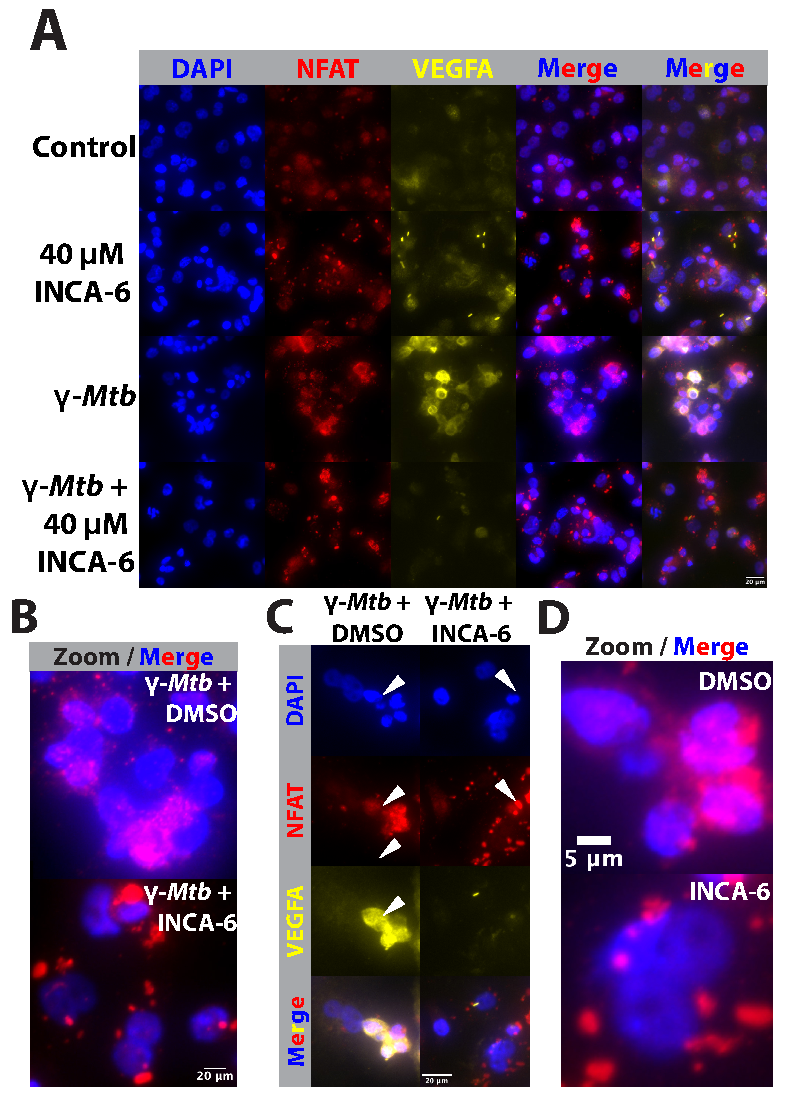
\includegraphics[height=5in]{images/incaIF.pdf}
\caption{Immunofluorescence imaging of gamma-irradiated \textit{M. tuberculosis} exposed THP-1 macrophages reveals robust NFAT protein translocation into the nucleus after exposure that corresponds to the induction of VEGFA. (A) shows robust VEGFA induction that can be inhibited by addition of INCA-6. (B) shows a magnified view of the NFAT nuclear translocation seen in (A). (C) shows further images and the correspondence between NFAT activation and VEGF production. (D) shows the reduction in nuclear localization from the images seen in (C).}
% Provide a label so we can cross-reference it from the tex
\label{figure:incaif}

\end{figure}

\begin{figure}
\centering
\includegraphics[width=\textwidth]{images/incaIFquant.pdf}
\caption{Quantitation of various aspects of the response seen by immunofluorescence after gamma-irradiated \textit{M. tuberculosis}-exposure and INCA-6 treatment. (A) shows the overall percentage of VEGFA+ cells seen in each condition, with a significant increase with $\upgamma$\textit{Mtb} exposure that is inhibited by INCA-6. (B) shows a parallel phenotype, where $\upgamma$\textit{Mtb} induces NFAT nuclear localization that is sensitive to INCA-6 addition. (C) shows the percentage of the total cells in the field of view that demonstrate both NFAT nuclear localization and VEGF expression.}
% Provide a label so we can cross-reference it from the tex
\label{figure:incaquant}
\end{figure}

\subsection{Requirement of human NFATC2 for VEGFA induction}\label{thp1lenti}

To identify functionally important NFAT human isoforms, we exposed THP-1 macrophages to $\upgamma$\textit{Mtb} and subsequently used the secretion inhibitor brefeldin A to lock VEGFA within secreting cells. Simultaneous staining for each of the four human NFATc proteins along with VEGFA allowed us to identify NFAT isoforms that underwent changes in expression and localization and correlate this with VEGFA production (\autoref{figure:isoforms}A). While THP-1 macrophages express all of the isoforms to varying degrees, the most intense co-staining with VEGF was found with NFATC2 (\autoref{figure:isoforms}B). Additionally, while each of the isoforms displayed sturctural and localization alterations (albeit not always nuclear) after $\upgamma$\textit{Mtb} exposure, only NFATC2 showed robust nuclear localization that appeared to correspond to VEGFA induction in individual cells (\autoref{table:isoforms}). While some NFAT isoform translocation was observable with at least NFATC1 and, somewhat, NFATC3, this generally had minor correspondence to the degree or presence of VEGFA production. While NFATC1 was correlated with VEGFA induction, the effect was much weaker than that seen with NFATC2. We quantified this effect by counting the number of VEGFA-expressing, NFAT nuclear localized cells and normalized to the number of VEGFA-expressing cells in total and found that NFATC2 most tightly corresponded to the induction of VEGFA in $\upgamma$\textit{Mtb}-exposed cells \autoref{figure:isoformsquant}. Given the strong correlation for NFATC2 with nuclear localization and VEGFA production after $\upgamma$\textit{Mtb} exposure, expression data from zebrafish and non-human primate granulomas, as well as the \textit{in vivo} zebrafish results implicating macrophage \textit{nfatc2a} in \textit{vegfaa} production and angiogenesis, we focused on human NFATC2 as the key isoform.

\singlespacing

\begin{center}
\begin{table}[h]
\caption{Lentiviral expression constructs to assess the role of NFATC2 domains for induction of VEGFA signaling.}
\label{table:isoforms} \tabularnewline
\vspace{0.5cm}
\begin{tabular}{|p{1in}|p{0.75in}|p{0.75in}|p{3in}|}
\hline
 & \thead{-$\upgamma$\textit{Mtb}} & \thead{+$\upgamma$\textit{Mtb}} & \thead{Relationship to VEGFA?} \tabularnewline
\hline
NFATC1 & + & ++ & Weak relationship between nuclear localization and VEGF expression. \tabularnewline
\hline
NFATC2 & ++ & +++ & Nuclear localization generally corresponds to VEGF expression. \tabularnewline
\hline
NFATC3 & + & ++ & Weak relationship between nuclear localization and VEGF expression. \tabularnewline
\hline
NFATC4 & +/- & + & Expression increased but not obviously nuclear in most cells. \tabularnewline
\hline
\end{tabular}
\end{table}
\end{center}

\doublespacing

\begin{figure}
\centering
\includegraphics[width=\textwidth]{images/isoformsIF.pdf}
\caption{To identify particular NFAT isoforms that may be important for VEGFA production downstream of \textit{M. tuberculosis} detection, immunofluorescence was performed against each of the isoforms. NFATC2 showed the most consistent induction of all of the isoforms. (A) shows alterations in the protein production and localization with and without \textit{M. tuberculosis}. (B) displays a representative field where multiple VEGFA-expressing cells can be seen, but only nuclear localization of NFATC2 seems to correspond with this expression.}
% Provide a label so we can cross-reference it from the tex
\label{figure:isoforms}
\end{figure}

\singlespacing

\begin{center}
\begin{table}[h]
\caption{Nearest gene neighbors for the ST sgRNAs (all are intergenic).}
\label{table:targets} \tabularnewline
\vspace{0.5cm}
\begin{tabular}{|p{1in}|p{4in}|}
\hline
\thead{sgRNA} & \thead{Nearest Gene Neighbor (Chromosome)} \tabularnewline
\hline
hU6 ST & CNTN1 (12) \tabularnewline
\hline
mU6 ST & MTDH (8) \tabularnewline
\hline
7SK ST & OPN5 (6) \tabularnewline
\hline
hH1 ST & ENSG00000249941 (5) \tabularnewline
\hline
\end{tabular}
\end{table}
\end{center}

\doublespacing

\begin{figure}
\centering
\includegraphics[height=3in]{images/NFAT_isoforms_110222.png}
\caption{We quantitated the immunofluorescence images from THP-1 macrophages stained with antibodies against the four NFAT isoforms to assess the contribution of each protein to the VEGFA expression phenotype. Indeed, we found that NFATC2 most tightly corresponded to VEGFA induction by measuring double positive cells (those with both VEGFA expression and NFAT nuclear localization) and normalized to the total number of VEGFA positive cells.}
% Provide a label so we can cross-reference it from the tex
\label{figure:isoformsquant}
\end{figure}

To test a functional role for human NFATC2 in macrophage induction of VEGFA during $\upgamma$\textit{Mtb} exposure, we used a lentivirus-mediated CRISPR/Cas9 approach to introduce high-efficiency disruption of NFATC2. Using techniques inspired by the zebrafish and backported to cell culture, we simultaneously expressed four distinct guide RNAs targeting NFATC2 or safe-targeting controls, to maximize the percentage of puromycin-resistant cells possessing complete null mutations \citep{Wu2018}. We compared these cells to those transduced with lentiviruses expressing safe-targeting control sgRNAs. (\autoref{figure:targets, table:targets}) \citep{Kabadi2014, Sanjana2014, Morgens2017, Kitamura2021}. Due to technical challenges associated with long-term culture of THP-1 cells and to address heterogeneity among cellular responses, we focused these assays on VEGFA induction in these cells by immunofluorescence after $\upgamma$\textit{Mtb} exposure. Because the N-terminal epitope recognized by our NFATC2 antibody was upstream of the targeted sites, we were unable to examine functional protein levels directly and simultaneously in the immunofluorescence images (\autoref{figure:validation}A). However, we found that transduced cells targeted by NFATC2 lentivirus generally failed to induce VEGFA while safe-targeting control lentivirus-transduced cells responded normally (\autoref{figure:lenti}A-B), an effect that can be quantitated by percentage of VEGFA+ cells by multiple metrics (\autoref{figure:lentiIFquant}A-C). These cells also demonstrated evidence of nonsense-mediated decay by NFATC2 transcript levels (\autoref{figure:validation}B). Thus, macrophage NFATC2-mediated induction of VEGFA downstream of mycobacterial TDM exposure is conserved from zebrafish to human cells exposed to \textit{M. tuberculosis}.

\begin{figure}
\centering
\includegraphics[height=2in]{images/lentitargets.pdf}
\caption{Based on our findings in THP-1 macrophages and the larval zebrafish, NFATC2 was selected for genetic targeting in the THP-1 macrophages. (A) displays the location of the four sgRNAs selected (in yellow arrows) and the location of the antibody epitope (red bar). (B) shows, on the genomic sequence itself, the location of the four sgRNAs.}
% Provide a label so we can cross-reference it from the tex
\label{figure:targets}
\end{figure}

\begin{figure}
\centering
\includegraphics[width=\textwidth]{images/lentiIF.pdf}
\caption{Lentivirus-mediated CRISPR/Cas9 targeting of NFATC2 results in reduced VEGFA expression after gamma-irradiated \textit{M. tuberculosis} exposure. (A) shows that Cas9-expressing NFATC2-targeted cells have a reduction in VEGFA production while similar Cas9-expressing cells with safe targeting control sgRNAs robustly induce VEGFA. (B) shows this magnified. Note the higher-expressing NFATC2-targeted cell has minimal Cas9 expression, suggesting that these effects may depend on the efficiency of targeting and other factors. (C) shows quantitation of the percentage of VEGFA+ cells in a given field of view, with a statistically significant reduction in the NFATC2-targeted condition.}
% Provide a label so we can cross-reference it from the tex
\label{figure:lenti}
\end{figure}

\begin{figure}
\centering
\includegraphics[height=3in]{images/lentivalid.pdf}
\caption{Validation of the lentivirus-mediated knockout approach. (A) shows aberrant localization of NFATC2, suggesting that the remaining protein has been functionally disrupted. Note that the antibody binding site is N-terminal to the sgRNA sites, a technical oversight in this design that made it difficult to quantify reductions in NFATC2 protein levels after targeting. (B) Nonsense-mediated mRNA decay in suspension THP-1 monocytes is reduced by NFATC2 targeting relative to safe targeting controls.}
% Provide a label so we can cross-reference it from the tex
\label{figure:validation}
\end{figure}

\begin{figure}
\centering
\includegraphics[width=\textwidth]{images/lentiIFquant.pdf}
\caption{Blinded quantification of our lentivirus-transduced CRISPR/Cas9 THP-1 macrophages demonstrating a reduction in the degree of VEGFA expression that corresponds to reduced NFATC2 nuclear responsiveness to $\upgamma$\textit{Mtb}. (A) shows the total percentage of VEGFA+ cells out of the total cells present. (B) is the percentage of cells with both VEGFA expression and NFATC2 nuclear translocation out of the total number of cells with NFATC2 nuclear translocation. (C) shows the percentage of the total number of cells that have both VEGFA expression and NFATC2 nuclear translocation. Together these data implicate NFATC2 in mediating the VEGFA response to $\upgamma$\textit{Mtb} exposure.}
% Provide a label so we can cross-reference it from the tex
\label{figure:lentiIFquant}
\end{figure}

\section{Discussion}\label{pap:disc}

This work uncovers an unexpected and novel role for macrophage NFAT activation in immune responses to pathogenic mycobacteria and the maladaptive angiogenic responses that occur during infection. This activation of NFAT is driven through recognition of bacterial cis\hyp{}cyclopropanated trehalose 6\hyp{}6'\hyp{}dimycolate, a major constituent of the cell envelope in pathogenic mycobacteria, that we have previously found is necessary and sufficient to drive pathological angiogenesis (Walton et al., 2018). Identifying this unexpected role for NFAT in angiogenesis expands our understanding of the mechanisms governing mycobacterial pathogenesis and offers targets for potential host directed therapeutics. Traditionally, work on TDM-mediated C-type lectin activation has focused on CARD9 and NF-$\upkappa$B signaling. Here, by contrast, we describe a specific role for alternative C-type lectin signaling responses through the NFAT pathway to drive VEGFA production and granuloma-associated angiogenesis. 

VEGFA induction is a prominent feature of tuberculosis in human disease as well as in a number of animal models, including non-human primates, rabbits, mice, and zebrafish \citep{Datta2015, Oehlers2015, Polena2016, Harding2019, Cronan2021, Gideon2022}. We found that VEGF was produced specifically within newly arrived macrophages at nascent granulomas. Macrophage populations are critical to VEGF induction, as macrophage-specific inhibition of NFAT signaling as well as deletion of \textit{nfatc2a} result in reductions in granuloma-associated angiogenesis. Using a human cell culture model, we found that NFATC2 was similarly engaged in human cells as amongst all NFAT isoforms, only NFATC2 underwent robust nuclear translocation in response to \textit{M. tuberculosis} stimulation. Correspondingly, pharmacological inhibition of NFAT signaling in human cell culture as well as genetic inhibition of \textit{NFATC2} resulted in reduced VEGFA production.

Although animal models of tuberculosis generally report high VEGF levels, there are few studies that center on VEGFA induction in cell culture infection models. Through high-resolution time-lapses and reporter lines, we found that \textit{vegfaa} induction generally does not occur until the formation of initial granulomas and is generally correlated with the appearance of extracellular bacteria that could be recognized by incoming, likely uninfected macrophages. This concentration-dependent effect on signaling may reflect key aspects of the disease itself, wherein large masses of extracellular bacteria accumulate in the necrotic core of the granuloma, potentially triggering relatively insensitive and/or chronic C-type lectin signaling in this context. Given what is already known about the need for chronic stimulus to produce effective NFATC2 activation, this would coherently fit with existing models and would offer a mechanism wherein other NFAT isoforms could play other roles earlier in infection but NFATC2 is specific to later stages at high intensity and duration of activation \citep{Yissachar2013, Kar2015}. 

Consistent with the recognition of extracellular bacteria, exposure of human macrophage-like cells to $\upgamma$-irradiated M. tuberculosis rapidly induced NFATC2-dependent VEGF signaling in a dose dependent manner. Standard cell culture infection models generally eliminate extracellular bacteria using gentamicin treatment and media changes, and so it is possible that engagement of this pathway by extracellular bacteria or TDM stimulation is a key component of this response. A survey of the literature and a variety \citep{Lee2019, Pisu2020, Hall2021, Looney2021, Pu2021} of RNA-seq datasets from macrophage-\textit{M. tuberculosis} infection experiments reveal modest or nonexistent induction of VEGFA, further supporting the notion that extracellular exposure to \textit{M. tuberculosis} may be an important element of the angiogenic response and may reflect some aspects of the macrophage-\textit{M. tuberculosis} interface within granulomas \citep{Orme2014b}.

As its name suggests, the NFAT pathway plays an indispensable role in normal T cell biology. Accordingly, whole animal knockouts of NFAT in standard mouse models of \textit{M. tuberculosis} infection --€“ where granuloma formation itself may be limited --€“ may have obscured a role for myeloid-specific effects of NFAT signaling \citep{Via2012}. This study investigated a role for NFATC2 in control of \textit{M. tuberculosis} infection and found that NFATC2 was required for effective bacterial control and production of TNF-$\upalpha$ and IFN-$\upgamma$ in CD4\textsuperscript{+} T cells despite no perturbation of the expression of these genes in dendritic cells, suggesting an adaptive immune response-specific defect in bacterial control. This may be of little surprise, given the extensive contacts that T cells have with mycobacteria within the lesions that develop in standard mouse models. Such a defect in T cell responses may be important for bacterial control when T cells are able to access the bacteria, but this condition is not reflective of the biology of the granuloma in other models or humans. It would be interesting to explore the phenotype of a \textit{LysM-Cre}; \textit{Nfatc2\textsuperscript{fl/fl}} mouse infected with tuberculosis to isolate the macrophage-dependent phenotypes. However, given our findings on macrophage NFAT contributions to angiogenesis, which is poorly modeled in the mouse, either entirely new roles for NFAT may be uncovered or it may have little or no effect on bacterial growth and disease. In any case, the present results offer some tension with these historical findings and it may take additional work to definitively identify any role for NFATC2 in the overall pathogenesis of tuberculosis infection.

The zebrafish model, by looking at early timepoints, uncovered a role both in angiogenesis and, presumably as a consequence, bacterial control. Wholesale, longer-term inactivation of NFAT, which also plays important roles in T cells, would compromise important aspects of a productive adaptive immune response during mycobacterial infection. While genetically manipulable animal models allow for cell-specific separation, any host-based therapeutic approaches might require cell-specific macrophage delivery methods \citep{Hu2019, Mukhtar2020, Colombo2022}, NFATC2-specific targeting \citep{Kitamura2021}, and/or contend with the adaptive immune response\footnote{Although NFATC2 appears to be largely redundant with both NFATC1 and NFATC2 for many, but not all adaptive responses, it is still important to, as specifically as possible, target the desired pathway for minimal off-target side effects.}, an important aspect of host resistance during mycobacterial infection.

While little else has been studied in the context of NFAT-mycobacterial interactions, a previous publication assessed the contributions calcineurin activation on the mycobactericidal activity of macrophages and found that mycobacteria manipulate an actin-binding protein called Coronin-1 to block phagosomal-lysosomal fusion and do so by activating calcineurin \citep{Jayachandran2007}. In the absence of Coronin-1 or after treatment with calcineurin inhibitors, lysosomes efficiently fused with the mycobacteria-containing phagosomes, mediating bacterial killing. This effect was found to be independent of transcription, implicating calcineurin in somehow modulating the process of phagosomal-lysosomal fusion, potentially through some interaction with Coronin-1 and actin. However, a subsequent publication found that this process was independent of actin \citep{Jayachandran2008}, leaving it a yet-to-be resolved mystery how directly calcineurin-dependent activity blocks phagosomal-lysosomal fusion to facilitate mycobacterial survival and replication. If nothing else, this adds to the body of evidence suggesting that calcineurin/NFAT-based host directed therapies may have multiple modes of host-beneficial activity.

It remains unclear why NFATC2, but not any of the other isoforms, is specifically required in macrophages for the induction of VEGFA, given evidence that the others are present in resting macrophages (\autoref{figure:isoforms}). The functional distinctions between the isoforms have long been of basic interest, but relatively few specific differences between them have been identified beyond basal regulation to provide tissue-specificity and more recent findings describing layers of kinetic regulation with isoform-specific stimulation thresholds, nuclear retention, and more \citep{Lyakh1997, Rao1997, Kar2014, Kar2015, Kar2016, Yissachar2013}. These novel levels of regulation offer opportunities for uncovering new features of the cell biology of NFAT.

NFAT is also likely to be involve in modulating the expression of other important pro-angiogenic chemokines, including CXCL12, the primary ligand for CXCR4. CXCR4 has been previously demonstrated to be critical for granuloma formation and angiogenesis \citep{Torraca2017} and NFAT has been shown to be able to regulate CXCL12 expression, at least in osteoblasts \citep{Sesler2013}. It may be reasonable to think that NFATC2 is also mediating CXCL12 expression during infection and is acting as a more central regulator of angiogenic responses. This hypothesis warrants further study; in any case, the stimulus for and transcriptional mediators of the observed CXCR4-dependent granuloma angiogenesis should be identified to add to our understanding of how these processes occur.

Here, we identify the unique requirement for this single isoform in macrophages to induce angiogenesis in response to mycobacterial infection. One hypothesis is that NFATC2 has binding partner(s) unique among NFAT isoforms required for its effect on the VEGFA promoter. Whether this is HIF-1$\upalpha$ (the canonical regulator of VEGFA) or one of the many previously described interacting partners is, as yet, unknown, but could be tested either \textit{in vitro} or \textit{in vivo} with genetic or chemical approaches. However, higher order regulatory mechanisms that result in the production of VEGF in the absence of overt hypoxia have been understudied and this work proposes at least one potentially generalizable mechanism whereby NFATC2 activation results in VEGFA transcriptional upregulation, a process that can be inhibited with chemical and genetic intervention. Despite the widespread presence of putative NFAT binding motifs (\seqsplit{5'€™-GGAAA-3'€™}) (\autoref{figure:promoter}) in the proximal VEGFA promoter \citep{Gearing2019}, their influence on VEGFA transcription has been relatively unexplored as this specific effect is generally not seen in T cells or other cell types \citep{Chang2004}. This single publication from \citet{Chang2004} found that the -2400 site in the \textit{VEGFA} promoter was specifically bound by NFATC proteins and acted to repress transcription. This is an intriguing hypothesis that might suggest that NFAT is able to repress \textit{VEGFA} transcription at baseline but may act to induce it after stimulation. Such results would be consistent with the mild but reproducible increase in VEGFA we observe with INCA-6 treatment in our experiments in THP-1 cells. 

As described in \autoref{NFAT}, NFAT is involved in the induction of a variety of cytokines including IFN-$\upgamma$ and TNF-$\upalpha$, but whether NFAT-dependent transcriptional induction of these within macrophages has a role in the overall course of disease is unknown. This surely offers promise for the future as an expansion of the present work to incorporate a more complete view of the NFAT-dependent signals that influence mycobacterial disease progression.

\begin{figure}
\centering
\includegraphics[width=\textwidth]{images/vegfapromoter.pdf}
\caption{NFATC2 and HIF-1$\upalpha$ putative binding sites in the VEGFA promoter as determined by CiiiDER. There are several NFAT binding sites in the promoter, the function of which has largely yet to be determined.}
% Provide a label so we can cross-reference it from the tex
\label{figure:promoter}
\end{figure}

A more comprehensive characterization of NFAT-dependent innate immune responses has begun in recent years \citep{Deerhake2021, Peuker2022, Poli2022} (for a more detailed description, see \autoref{nouveaunfat}), but this pathway has remained unstudied in the context of macrophage signaling during mycobacterial infection. Furthermore, this work draws a connection between the induction of calcium fluctuations --€“ which can occur in response to many different developmental, homeostatic, and pathological stimuli, including to mycobacterial infection \citep{Kusner2001, Jayachandran2007, Jayachandran2008, Matty2019, Malik2000} --€“ to the angiogenic response to that stimulation. Our identification of NFAT regulation of VEGFA offers a novel approach to both pro- and anti-angiogenic intervention in various pathological contexts.

\subsection{Limitations of the Study}

The limitations of this study are innumerable. While I am proud of what I have accomplished in pursuit of this work, there are many opportunities for the future as well as further work to clarify the results we have found here. We have identified interesting macrophage biology mediating an important disease-relevant phenotype during mycobacterial infection, but we do not see the same magnitude of bacterial burden change as with VEGF-inhibition alone \citep{Oehlers2015}, suggesting pleiotropy in the NFAT signaling pathway with inhibition resulting in both pro- and anti-bacterial effects. What these antimycobacterial aspects of NFAT signaling are is worth investigation to better understand the full corpus of possible consequences to NFAT inhibition strategies for the treatment of infectious disease and the potential risks for patients already taking calcineurin inhibitors. To do so, RNAseq or similar should be employed to better delineate these alterations in gene expression profile.

We have thus far been unable to identify the particular macrophage receptor responsible for detecting TDM in the zebrafish. While work in THP-1 macrophages may be able to more affirmatively link MINCLE or MCL to the activation of NFAT, identification of the zebrafish receptor would make a substantive contribution to model development as well as the evolution of C-type lectin receptors more broadly. Cell-type specific knockout of \textit{nfatc2a} would also aid greatly in definitively linking this gene to VEGFA induction and angiogenesis, but the tools to do so are not yet operational; perhaps future studies can begin with such intent and focus more stringently on the role of this isoform strictly in macrophages.

Some technical limitations are also interfering with interpretation of some results. Generation of stable knockouts of NFATC2 in THP-1 macrophages would make for more robust and cleaner assays, although it has the limitation of odd clonal behavior and loses the heterogeneity that can be advantageous in dissecting some phenotypes. The variable ploidy of these cells is also a challenge, so an alternative macrophage model or primary cells may be required to more effectively model some of these responses.

This macrophage-NFAT signaling pathway likely has important roles in other disease contexts that are not addressed here. Tuberculosis is the most common cause of granuloma formation, but it is far from the only cause, and any contributions of this pathway to granuloma biology in \textit{Schistosoma}, \textit{Cryptococcus}, or \textit{Histoplasma} infections is not yet known. However, with the tools now available, these roles are likely to be easier to study in the future and new insights may be gleaned from such investigation. Angiogenesis is a common pathology in some autoimmune diseases, such as arthritis, and is prevalent among cancers; whether macrophage NFAT signaling might be mediating angiogenesis in these contexts is surely of future interest and may reveal novel aspects of the host-tumor interface.

We have validated important aspects of our observations in the zebrafish with a mammalian cell culture model, but subsequent studies may warrant further integration of mammalian models of tuberculosis infection where angiogenesis is present (rabbits, guinea pigs, macaques) or human patient samples to better understand certain aspects of the underlying biology and validate NFAT induction during tuberculosis infection and potential correspondence to VEGFA production.

